\section{插入图片}
\subsection{常用参数说明}
\subsubsection{位置偏好}
使用 \texttt{figure} 宏包插入图片时,可通过 \latex{\begin{figure}[OPTION]} 中的 \texttt{OPTION} 指定插入图片的位置偏好。

\begin{itemize}
    \item \texttt{h} 源码中近似相同的位置(here)
    \item \texttt{t} 页面上方(top)
    \item \texttt{b} 页面底部(bottom)
    \item \texttt{p} 单独占据一页(page)
    \item \texttt{!} 覆盖 \LaTeX 所认为的合适位置
    \item \texttt{H} 源码中精确相同的位置,类似于 \texttt{h!}
\end{itemize}

注意前四个标识仅表示偏好,当 \LaTeX 认为如此放置图片不合适时,可以选择不遵从指定的偏好。一般使用 \texttt{htbp} 或 \texttt{hbt!} 等偏好组合,\LaTeX 将会尽量满足优先度更高的偏好,除非用户要求强制执行。

\subsubsection{修改图片}
使用 \latex{\includegraphics[OPTION]{filename}} 命令插入图片时,可单独或组合使用如下参数。

\begin{itemize}
    \item \texttt{scale=2.0} 对照原图大小的等比例缩放因子
    \item \texttt{width=3cm} 指定图片宽度
    \item \texttt{height=4cm} 指定图片高度
    \item \texttt{angle=45} 逆时针旋转度数
\end{itemize}

注意以上数值可指定精确的单位数值,如点宽 \texttt{pt}、毫米 \texttt{mm}、厘米 \texttt{cm}、英寸 \texttt{in}、字母\texttt{x}的高度 \texttt{ex}、字母 \texttt{m}的宽度 \texttt{em};也可根据内置变量指定,如列间距 \latex{\columnsep}、列宽 \latex{\columnwidth}、行宽 \latex{\linewidth}、页宽 \latex{\paperwidth}、页高 \latex{\paperheight}、字宽 \latex{\textwidth}、字高 \latex{\textheight}、图片单位长度 \latex{\unitlength}。


\newpage
\subsection{单张图片}
使用如下代码,效果如图 \ref{fig:single}。

\inputminted{latex}{src/image-single.tex}
\begin{figure}[htbp]
\centering
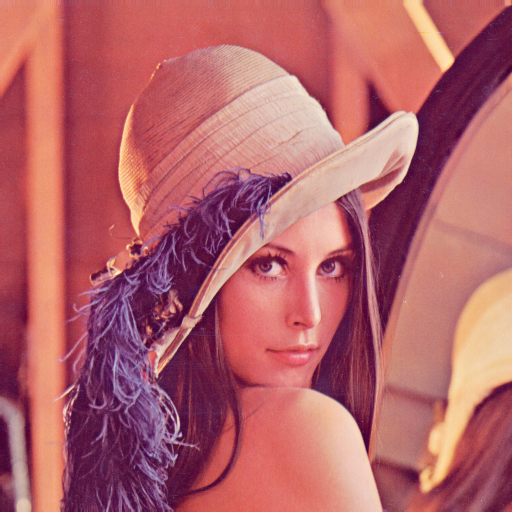
\includegraphics[width=10cm]{img/lena.png}
\caption{插入单张图片}
\label{fig:single}
\end{figure}


\newpage
\subsection{多张图片(独立编号)}
使用 \texttt{minipage} 宏包和如下代码,效果如图 \ref{fig:double:left} 和图 \ref{fig:double:right}。

\inputminted{latex}{src/image-double.tex}
\begin{figure}[htbp]
  \begin{minipage}{0.5\linewidth}
    \centering
    
\includegraphics[width=0.9\linewidth]{img/peppa.jpg}
    \caption{佩琦}
    \label{fig:double:left}
  \end{minipage}
  \begin{minipage}{0.5\linewidth}
    \centering
    
\includegraphics[width=0.9\linewidth]{img/george.jpg}
    \caption{乔治}
    \label{fig:double:right}
  \end{minipage}
\end{figure}


\newpage
\subsection{多张图片(共同编号)}
使用 \texttt{subfigure} 宏包和如下代码,效果如图 \ref{fig:subfig} 中的图 \ref{fig:subfig:1}、\ref{fig:subfig:2} 等。

\inputminted{latex}{src/image-subfig.tex}
\begin{figure}[htbp]
\centering
\subfigure[爸爸]{
	\label{fig:subfig:1}
	
\includegraphics[width=0.45\linewidth]{img/dad.jpg}
}
\hspace{0.01\linewidth}
\subfigure[妈妈]{
	\label{fig:subfig:2}
	
\includegraphics[width=0.45\linewidth]{img/mom.jpg}
}
\vfill
\subfigure[爷爷]{
	\label{fig:subfig:3}
	
\includegraphics[width=0.45\linewidth]{img/grandpa.jpg}
}
\hspace{0.01\linewidth}
\subfigure[奶奶]{
	\label{fig:subfig:4}
	
\includegraphics[width=0.45\linewidth]{img/grandma.jpg}
}
\caption{佩琦的长辈们}
\label{fig:subfig}
\end{figure}

